\input format.tex

\usepackage{graphicx}
\graphicspath{{cores/}}

\begin{document}

\vspace*{5mm}
%% 各章节
\setlength{\arrayrulewidth}{1pt}
\fontsize{9.3pt}{11pt}\selectfont
\color{gray2}

\centerline{\bf\sanhao 健康建议}

\vspace*{2mm}

\begin{LRaside}[.20]{膳食方案}
{\bf *综合您肠道菌群检测结果,为您定制以下膳食方案:}\\
{\indent 建议低脂、低糖、低热量饮食,控制总能量的摄入。规律进餐,细嚼慢咽。控制主食量,主食以燕麦、薯类等粗粮为主。蛋白质宜选用鸡蛋、鱼虾及豆制品等优质蛋白。多食用含糖低并富含膳食纤维的果蔬,如芦笋、芹菜、洋葱等。少油少盐,食用油控制在每天25克以内,食盐控制在每天6克以内。忌肥肉、油炸等高脂食物。忌含糖饮料。忌暴饮暴食。如患痛风、溃疡性结肠炎、慢性腹泻、食物不耐受等有饮食禁忌的疾病,请综合考虑疾病的饮食原则。}\\
\asidebreak %
\noindent

\includegraphics[width=\linewidth]{shanshifangan.pdf}

\end{LRaside}


\begin{LRaside}[.70]{营养调节方案}
\noindent

\includegraphics[width=\linewidth]{tiaojiefangan.pdf}

\asidebreak %
{\bf *综合您肠道菌群、营养功能检测结果,为您定制以下营养调节方案:}\\
{\bf 调节肠道菌群、补充营养}\\{\indent 1.每天选择性补充膳食纤维咀嚼片。膳食纤维可减少人体能量摄入,减少肠道对糖类和脂肪的消化吸收。 

2.选择性补充低聚果糖类益生元产品,可以促进排泄物的排出,减少有害物质在体内的存留时间。(如患炎症性肠病、慢性腹泻,不宜服用菊粉及低聚果糖,建议选择低聚半乳糖。)

3.可选择性补充复合蛋白固体饮料、大豆肽蛋白粉、含有几丁聚糖的保健品,帮助您控制体重。}\\
\end{LRaside}

\begin{LRaside}[.20]{运动方案}
{\bf *适量运动可以帮助改善肠道菌群}\\
{\indent 条件允许的情况下,选择爬楼梯,自行车出行等方式锻炼身体。多参加团体运动,培养运动习惯。建议选用持续时间长、低强度的运动方式,如快步走、慢跑、骑自行车、游泳、乒乓球、羽毛球、网球、健身操等。配合增加肌肉量的运动,如俯卧撑、哑铃、深蹲等。建议早饭或晚饭前空腹状态下进行运动,每次运动时间30分钟以上,每周5次以上。}
\asidebreak %
\noindent
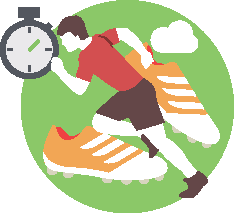
\includegraphics[width=\linewidth]{yundongfangan.pdf}

\end{LRaside}

%\vspace*{0.5mm}
{\noindent\qihao *以上健康建议仅供参考,您的实际饮食、保健、运动等还需结合自身具体情况。}

\end{document}
